%
\pdfoutput=1
\pdfminorversion=5 % necessary for EES
%
%\documentclass[12pt,number,sort&compress,preprint,review]{elsarticle}
\documentclass[smallextended,referee]{svjour3}

\smartqed

\journalname{}
% better printing of numbers
\usepackage[utf8]{inputenc}
\usepackage[T1]{fontenc}
\usepackage[english]{babel}
\usepackage{graphicx}
\usepackage{latexsym, amsmath, amssymb}
\usepackage{listings}
\usepackage{float}
\usepackage{hyperref}
\usepackage{enumitem}
\usepackage{tcolorbox}
\usepackage{subcaption}
\hypersetup{
    colorlinks=true,
    linkcolor=blue,
    filecolor=magenta,      
    urlcolor=cyan,
}


      

\newenvironment{codeblock}[1]
{
\begin{figure}[hbt]
\newcommand{\captionMacro}{#1}
\centering
\begin{tcolorbox}[width=15cm]
}
{
\end{tcolorbox}
\caption{\captionMacro{}}
\end{figure}
}



\begin{document}


\title{Modeling atmospheric chemistry using Cantera reactor networks.}

\titlerunning{Modeling atmospheric chemistry using Cantera reactor networks.}

\author{Anthony S.~Walker}

\institute{A.~Walker \at
           School of Mechanical, Industrial, and Manufacturing Engineering, Oregon State University, Corvallis, OR, USA \\

           \email{walkanth@oregonstate.edu}
}
\date{Received: date / Accepted: date}
\def\pyplume{\texttt{PyPlume}}
\def\SCALE{0.5}

\maketitle 

\begin{abstract}
As society continues to relay on the burning of fuel to extract energy, it is important to understand the impact that our actions have on our health and the environment. \pyplume{} is a software developed for the purpose of modeling exhausts to help understand these impacts. The software focuses on building complicated reactor networks to more practically simulate the exhaust-atmosphere interaction and understand the composition and effects of exhaust products on the environment. The software is the result. A tool that can be used for further study based on a researcher's needs. 
\end{abstract}


\section{Introduction}

Chemistry plays an important role in many aspects of today's society such as transportation, healthcare, energy production, and environmental safety and protection. As society continues to relay on the burning of matter to extract energy, it is important to understand the impact that our actions have on our health and the environment. Is all the fuel we burn detrimental to our health in the long term? To what degree can we safely continue our way of life? Are we destroying other forms of life on the planet as well with out behavior? The list of important questions goes on and answering them is no minor feat.


Answering these questions definitively requires scientific study to develop and model the lifespan and behavior of products from burning matter. Small scale phenomena can be analyzed experimentally to determine constituents and potential impacts. However, how do you experimentally model wildfire that burns hundreds of thousands of acres with an immense variety of different fuels both living and dead? How do you model the burning of a jet fuel which has thousands of different chemical species to track? How do you follow the products from both scenarios throughout the atmosphere across the world? The answer would seem to be computational modeling, but it has it's limitations as well. First and foremost, modeling such complicated phenomena requires a lot of computing resources. The models can be simplified to use less resources but at the cost of accuracy.

Aircraft contrails are a large contributor to radiative forcing

\section{Motivation}


\section{Methods}

\pyplume{} was built with Cantera\cite{cantera} at it's core. The goal was to create a versatile \texttt{Python} tool that can generate complicated exhaust models with a reactor network approach. While complicated models are currently constrained by expense, I am working towards implemented methods to drastically accelerate the solution process and reduce this expense. This package was created with the intention of using these methods on a particular application such as a more rigorous study of aircraft exhaust. \pyplume{} focuses on the exhaust portion of the system but also includes a reservoir-combustor network to generate the input conditions and, an atmospheric reservoir for mass entrainment into the exhaust network. The general idea is shown in Figure~\ref{fig:general}.

\begin{figure}[htb!]
    \centering
    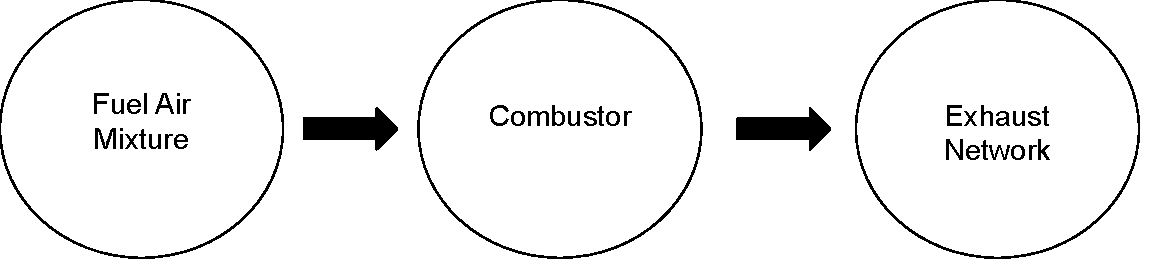
\includegraphics[scale=\SCALE]{examples/report/figures/general.pdf}

    \caption{General concept for modeling exhaust networks in pyplume.}
    \label{fig:general}
\end{figure}

So, how do we produce a more in-depth study with a set of well-stirred ideal gas reactors? The main idea that I had was the ability to relax the well mixed nature of well-stirred reactors. This can be achieved with multiple connected reactors, entrainment, and mass conservation. \pyplume{} uses an adjacency matrix approach to creating and connecting the exhaust reactor network which makes this possible, e.g., mass entrainment into an outer reactor will provide a different concentration than inner reactors. The second idea was to use larger mechanisms that include more of elementary reactions. This is also possible with the package because the mechanism can be independently specified for every reactor if desired. 

These ideas led to the development of three models within \pyplume: \texttt{simple}, \texttt{linear}, and \texttt{grid}. The simple model was used primarily in developing and testing and is shown in Figure~\ref{fig:simple}. 

\begin{figure}[htb!]
    \centering
    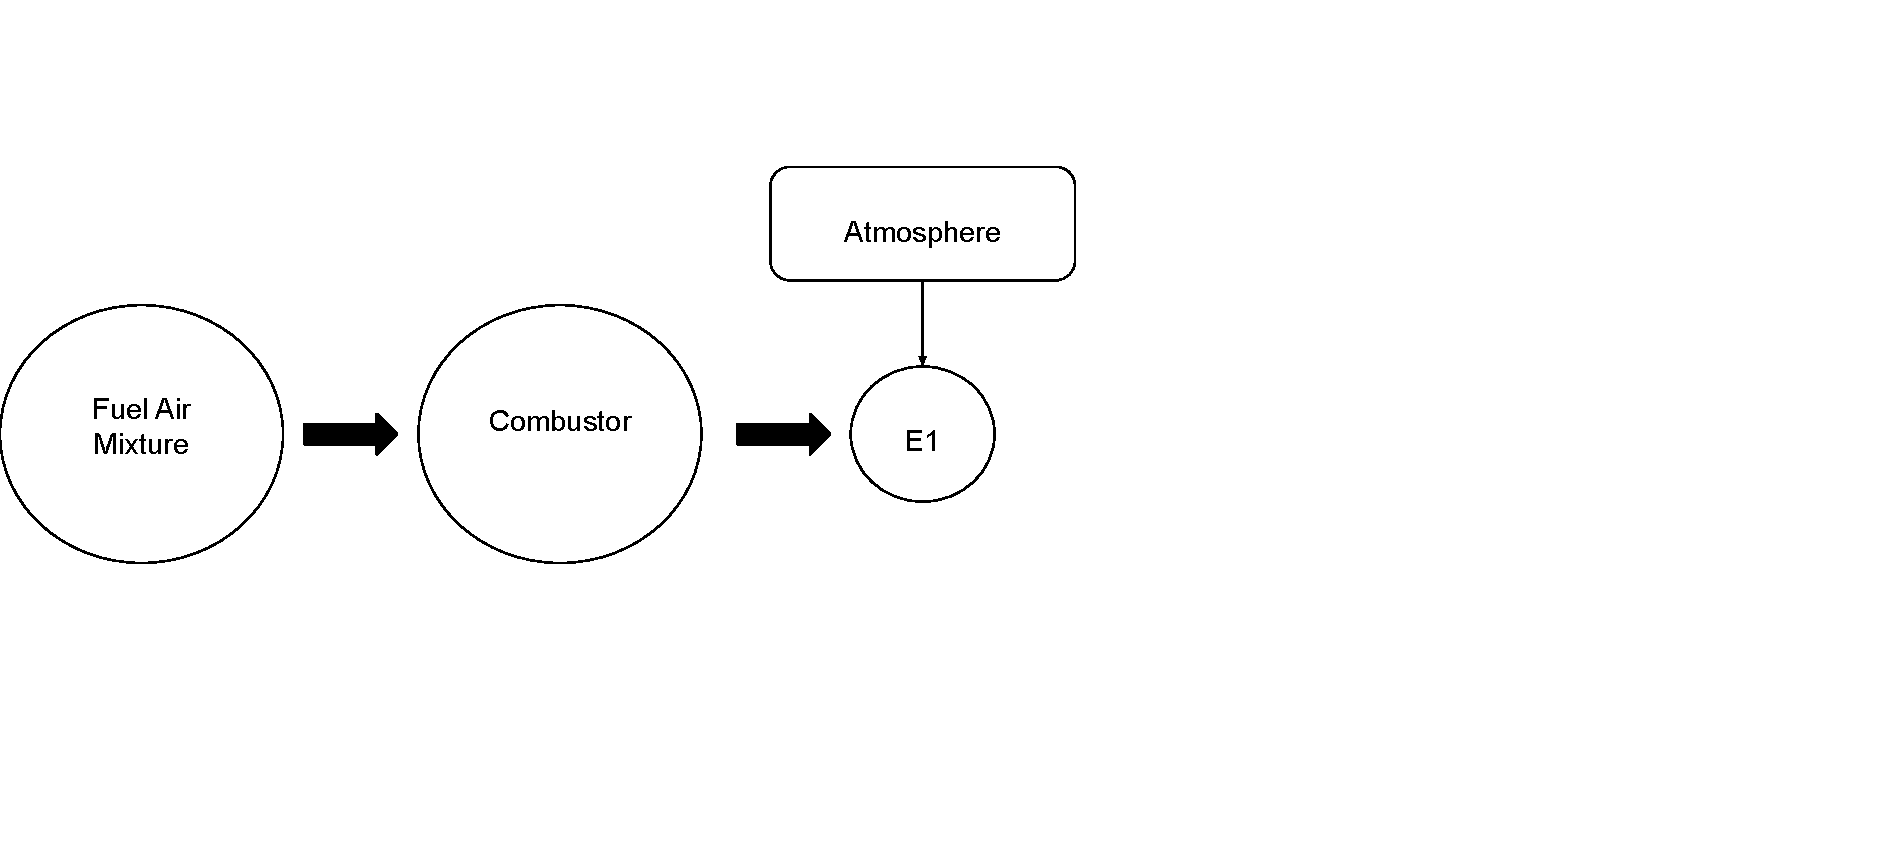
\includegraphics[scale=\SCALE,trim=1cm 5cm 1cm 4cm]{examples/report/figures/simple.pdf}

    \caption{Simple model for testing and developing.}
    \label{fig:simple}
\end{figure}

The \texttt{grid} and \texttt{linear} models were developed as different takes on achieving a less well mixed system but they have yet to be formally tested and verified to this end. These models aside, \pyplume{} can be used to develop other models by providing an adjacency matrix to the software. I suspect this will be the the most useful for my application. For example, to produce the \texttt{linear}, and \texttt{grid} model shown in Figures~\ref{fig:linear} and \ref{fig:grid}, the adjacency matrices would respectively be 
\setcounter{MaxMatrixCols}{12}
\renewcommand*{\arraystretch}{0.5}
\begin{equation*}
    \begin{bmatrix}
     0 & 1 & 1 & 0 & 0 & 0 & 0 & 0 & 0 & 0 & 0 \\
     0 & 0 & 0 & 1 & 1 & 1 & 0 & 0 & 0 & 0 & 0 \\
     0 & 0 & 0 & 1 & 1 & 1 & 0 & 0 & 0 & 0 & 0 \\
     0 & 0 & 0 & 0 & 0 & 0 & 1 & 1 & 1 & 1 & 0 \\
     0 & 0 & 0 & 0 & 0 & 0 & 1 & 1 & 1 & 1 & 0 \\
     0 & 0 & 0 & 0 & 0 & 0 & 1 & 1 & 1 & 1 & 0 \\
     0 & 0 & 0 & 0 & 0 & 0 & 0 & 0 & 0 & 0 & 0 \\ 
     0 & 0 & 0 & 0 & 0 & 0 & 0 & 0 & 0 & 0 & 0 \\ 
     0 & 0 & 0 & 0 & 0 & 0 & 0 & 0 & 0 & 0 & 0 \\ 
     0 & 0 & 0 & 0 & 0 & 0 & 0 & 0 & 0 & 0 & 0 \\ 
     1 & 1 & 1 & 1 & 0 & 1 & 1 & 0 & 0 & 1 & 0 
    \end{bmatrix}\quad and\quad
    \begin{bmatrix}
     0 & 1 & 1 & 1 & 0 & 0 & 0 & 0 & 0 & 0 & 0 \\
     0 & 0 & 0 & 0 & 1 & 0 & 0 & 0 & 0 & 0 & 0 \\
     0 & 0 & 0 & 0 & 0 & 1 & 0 & 0 & 0 & 0 & 0 \\
     0 & 0 & 0 & 0 & 0 & 0 & 1 & 0 & 0 & 0 & 0 \\
     0 & 0 & 0 & 0 & 0 & 0 & 0 & 1 & 0 & 0 & 0 \\
     0 & 0 & 0 & 0 & 0 & 0 & 0 & 0 & 1 & 0 & 0 \\
     0 & 0 & 0 & 0 & 0 & 0 & 0 & 0 & 0 & 1 & 0 \\
     0 & 0 & 0 & 0 & 0 & 0 & 0 & 0 & 0 & 0 & 0 \\
     0 & 0 & 0 & 0 & 0 & 0 & 0 & 0 & 0 & 0 & 0 \\
     0 & 0 & 0 & 0 & 0 & 0 & 0 & 0 & 0 & 0 & 0 \\
     1 & 1 & 0 & 1 & 1 & 0 & 1 & 1 & 0 & 1 & 0 
 \end{bmatrix}.
\end{equation*}

These adjacency matrices could be further used to specify reverse flow into reactors, i.e., moving upstream. While it has not been tested in this scenario, it is possible. These connections are \texttt{MassFlowController} objects from \texttt{Cantera} and continuity is maintained in a simple manner, i.e., mass flow out of a reactor is divided by the number of sinks. 
\begin{equation}
    \dot{m}_i = \frac{m_i}{n_{s,i} \tau (t)},
\end{equation}

\begin{figure}[htb!]
    \centering
    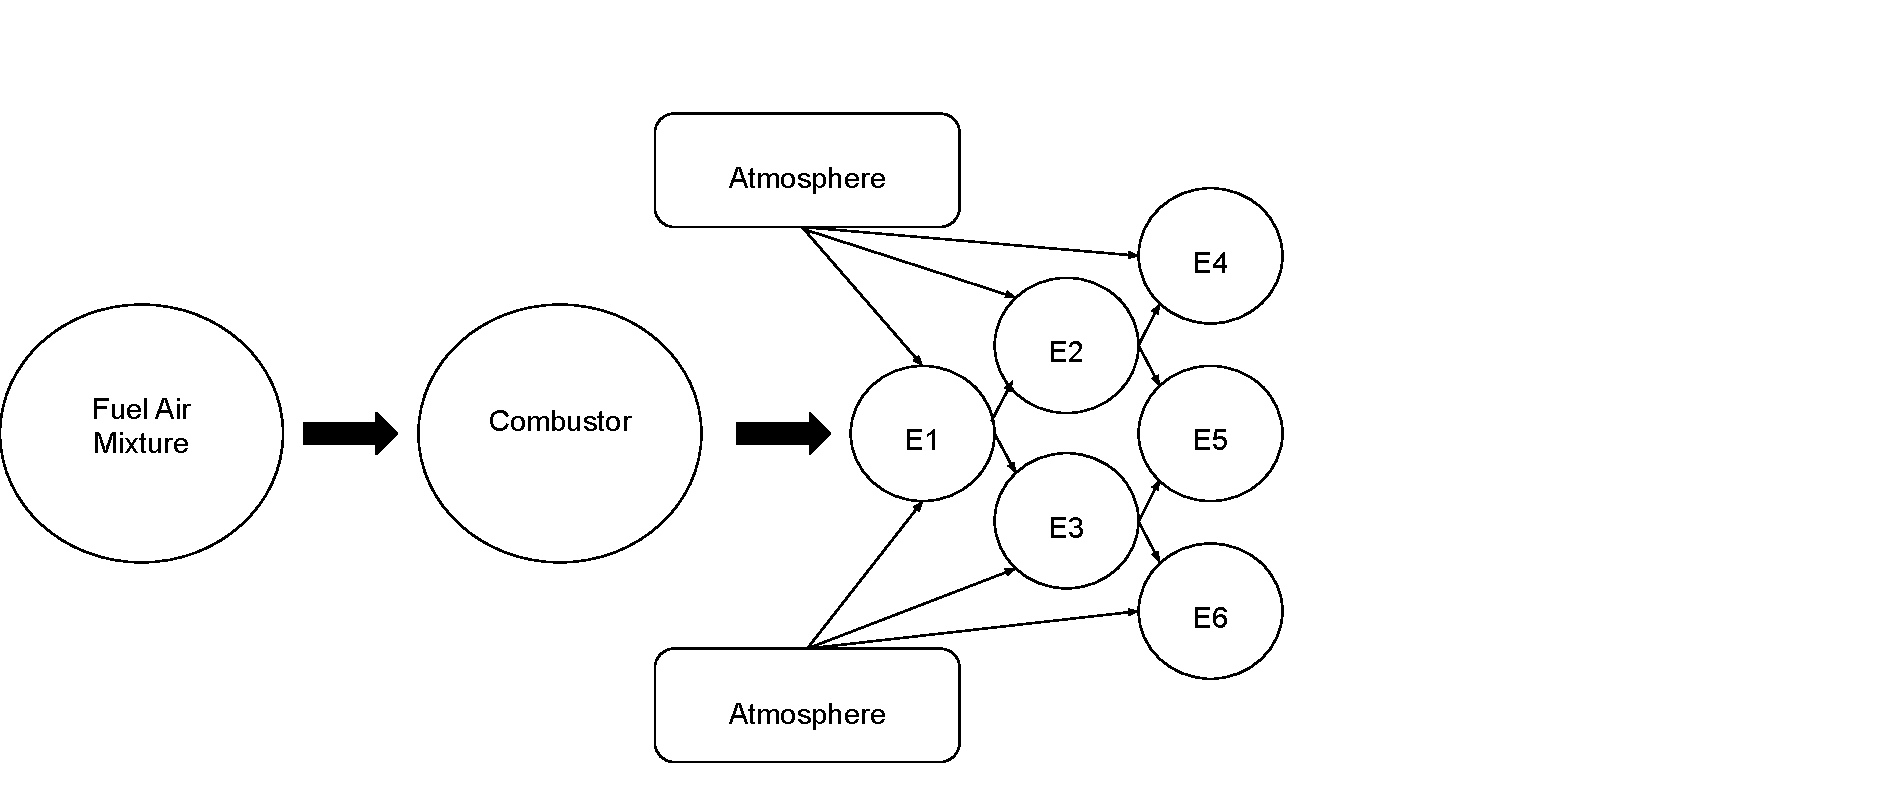
\includegraphics[scale=\SCALE,trim=1cm 1cm 1cm 1cm]{examples/report/figures/linear.pdf}

    \caption{Linear model for developing a less well mixed system.}
    \label{fig:linear}
\end{figure}

where $\dot{m_i}$ is the mass flow from a specific reactor, $m_i$ is mass of that reactor, $n_{s,i}$ is the number of sinks for that reactor, and $\tau(t)$ is the residence time as a function of clock time. $\tau(t)$ is specified, $m_i$ is also determine from an initial specified value but evolves throughout the simulation, and $n_{s,i}$ is the sum of the $i^{th}$ row of the adjacency matrix. The details of this can be found in the \texttt{model.py} file of the package.

\begin{figure}[htb!]
    \centering
    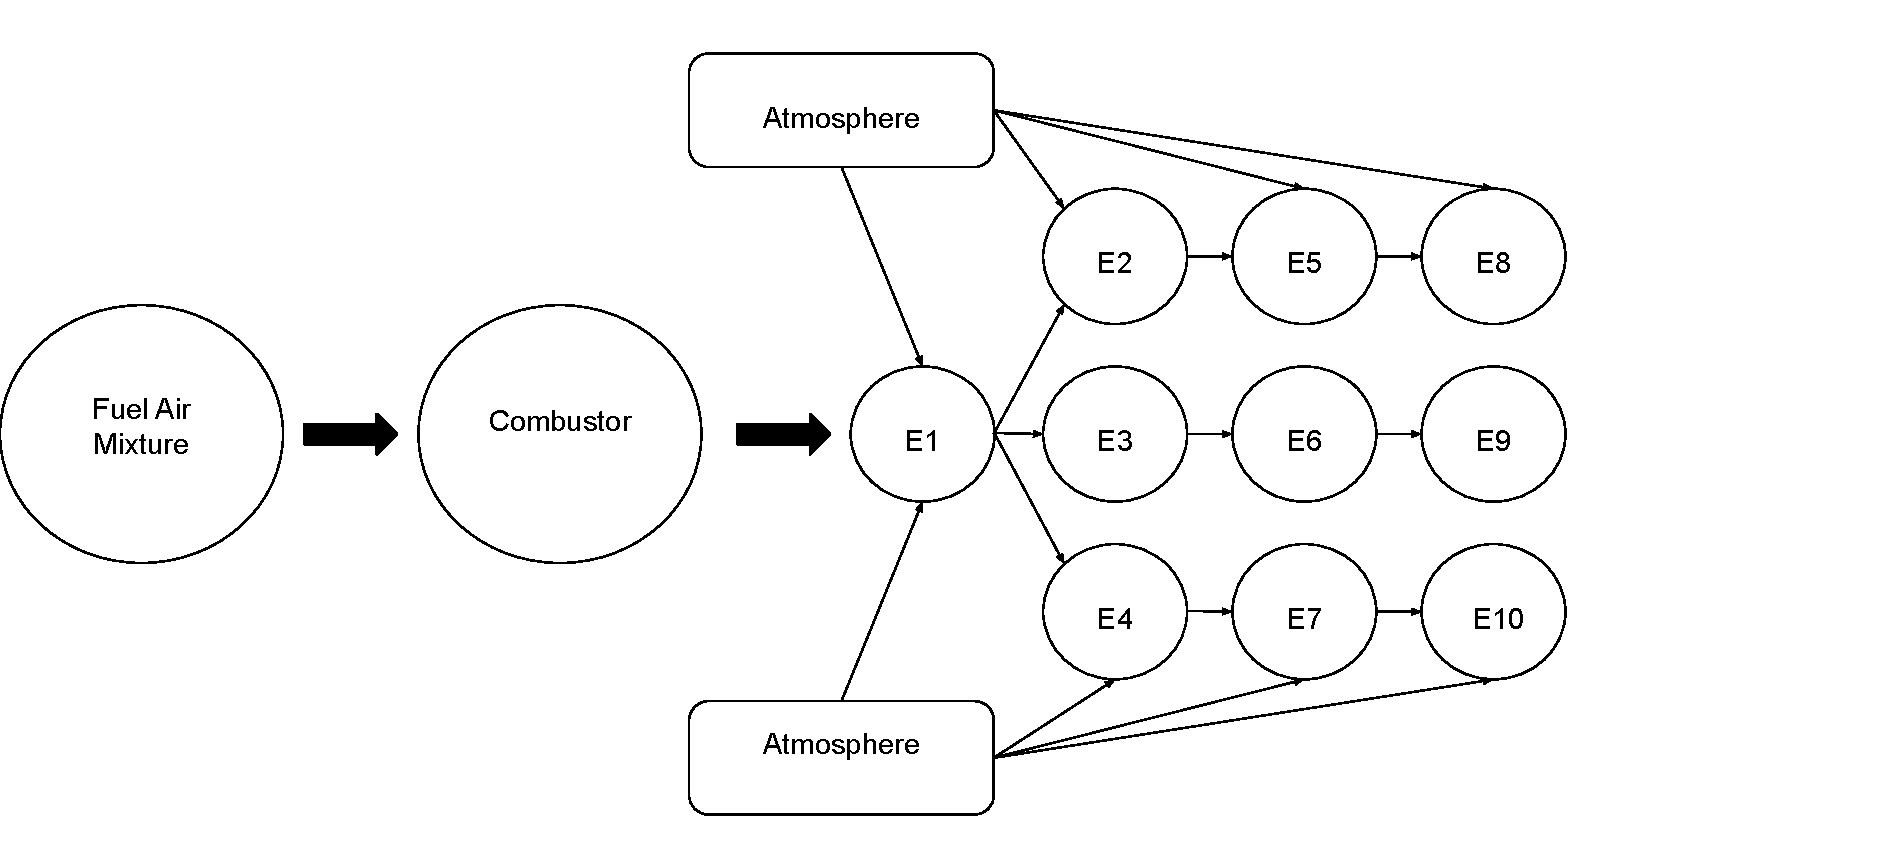
\includegraphics[scale=\SCALE,trim=1cm 1cm 1cm 1cm]{examples/report/figures/grid.pdf}

    \caption{Grid model for developing a less well mixed system.}
    \label{fig:grid}
\end{figure}

The modeling is the primary function of \pyplume{} but it also has other functionalities. It includes methods for plotting data and constituents from the reactor network in various combinations based on user input. It includes methods for testing the currently implemented code, and it also has a command line interface for all of the currently implemented modules. The methods used in the modules are not necessarily critical to this section but more of added functionality---so I omitted discussion of them here.




\section{Results}
The major result of this project is \pyplume{} itself. During development, it was not applied to a specific application but built for future needs of my project. So this section will focus on it's use as it is the primary result. The source code for \pyplume{} is available on \href{https://github.com/SoftwareDevEngResearch/pyplume}{Github}\footnote{\url{https://github.com/SoftwareDevEngResearch/pyplume}}. It is also available at on \href{https://pypi.org/project/pyplume/}{PyPi}\footnote{https://pypi.org/project/pyplume/} and \href{https://anaconda.org/anthony-walker/pyplume}{Anaconda}\footnote{https://anaconda.org/anthony-walker/pyplume}.

I believe the easiest way to use \pyplume{} through \texttt{conda} via
\\
\noindent
\texttt{conda install -c anthony-walker -c cantera -c conda-forge pyplume}.
\pyplume{} has five submodules, four of which are fully implemented for the current version:
\begin{enumerate}[noitemsep,topsep=0pt]
    \item \texttt{pyplume.mech}
    \item \texttt{pyplume.model}
    \item \texttt{pyplume.figures}
    \item \texttt{pyplume.output}
    \item \texttt{pyplume.statistics} - (not fully implemented)
\end{enumerate}
\noindent
All of these submodules have both a command line and a script interface.

\subsection{\textbf{Command line}}

In this section, I will walk through use on the command line. The \texttt{mech} package offers capabilities to manage your mechanism files as well as use mechanisms already provided by the package. \texttt{pyplume.mech -h} will show all of the available options to the user---Figure~\ref{code:mech}. Use of this package however is completely optional; Cantera provides a built in set of mechanism files which can be used with the \texttt{model} interface.

\begin{codeblock}{Commandline interface help for \texttt{pyplume.mech}}
\begin{lstlisting}[language=bash]
usage: pyplume.mech [-h] [-r] [-l] [-a ADD] [-d DELETE] [-t]
This is the commandline interface for managing mechanism files of PyPlume.
optional arguments:
  -h, --help            show this help message and exit
  -r, --restore         set this flag to restore mechanism files.
  -l, --list            set this flag to list mechanism files.
  -a ADD, --add ADD     this can be used to add a mechanism file to the codes
                        internal data.
  -d DELETE, --delete DELETE
                        this can be used to delete a mechanism file to the
                        codes internal data.
  -t, --test            set this flag to run test functions.
\end{lstlisting}
\label{code:mech}
\end{codeblock}

The model interface---shown in Figure~\ref{code:model}---can be used with \texttt{pyplume.model -h}. It has one positional argument which requires a specified model (\texttt{simple}, \texttt{grid}, \texttt{linear}). Otherwise, it gives the capabilities to run a simulation as desired based on certain flags.

\begin{codeblock}{Command line interface help for \texttt{pyplume.model}}
\begin{lstlisting}[language=bash]
usage: pyplume.model [-h] [-ss] [-t0 [T0]] [-tf [TF]] [-m [MECH]] [-dt [DT]]
                     [-t] [-v]
                     [{simple,grid,linear}]
This is the commandline interface for running an exhaust network.
positional arguments:
  {simple,grid,linear}  This is a required arguement that specifies the model
                        which will be used. Currently implemented choices are
                        simple, grid, and linear.

optional arguments:
  -h, --help            show this help message and exit
  -ss, --steady         set this flag run to steady state after integration
  -t0 [T0]              Initial integration time
  -tf [TF]              Final integration time
  -m [MECH], --mech [MECH]
                        mechanism file
  -dt [DT]              Integration time interval
  -t, --test            set this flag to run test functions.
  -v, --verbose         set this flag to run print statements during the
                        process.
\end{lstlisting}
\label{code:model}
\end{codeblock}

The final interface available to the command line is \texttt{pyplume.figures -h}---shown in Figure~\ref{code:figures}. This interface allows the plotting of data produced by the \texttt{pyplume.model} interface.

\begin{codeblock}{Command line interface help for \texttt{pyplume.figures}}
\begin{lstlisting}
usage: pyplume.figures [-h] [-t] [-v] [-w] [-d] [-p PROPERTY [PROPERTY ...]]
                       [-r REACTORS [REACTORS ...]]
                       [filename]
This is the commandline interface for plotting results from the exhaust
network.
positional arguments:
  filename              filename used for plotting.

optional arguments:
  -h, --help            show this help message and exit
  -t, --test            set this flag to run test functions.
  -v, --verbose         set this flag to run corresponding print statements
                        through code.
  -w, --write           write plots to file as they are generated.
  -d, --display         set this flag to display plots on screen.
  -p PROPERTY [PROPERTY ...], --property PROPERTY [PROPERTY ...]
                        Plot a specific property
  -r REACTORS [REACTORS ...], --reactors REACTORS [REACTORS ...]
                        Specify reactors integer indices to plot property for
                        a subset of reactors

\end{lstlisting}
\label{code:figures}
\end{codeblock}

These three interfaces can be combined to produce data and figures as desired. This example creates places \texttt{test.cti} in the mechanism files (assuming that it exists in the directory). It then integrates to the final time of 1, advances to steady state, and plots the resulting data.

\begin{codeblock}{Usage of CLI interface on an example}
\begin{lstlisting}
pyplume.mech -a test.cti
pyplume.model simple -tf 1 --steady --verbose --mech test.cti
pyplume.figures simple.hdf5 -d -w -p 'CO2' 'mass'
\end{lstlisting}
\label{code:CLI}
\end{codeblock}

The resulting data was omitted for brevity purposes but the plots generated are shown in Figure~\ref{fig:plots}.

\begin{figure}[ht]
\begin{subfigure}{.6\textwidth}
  \centering
  % include first image
  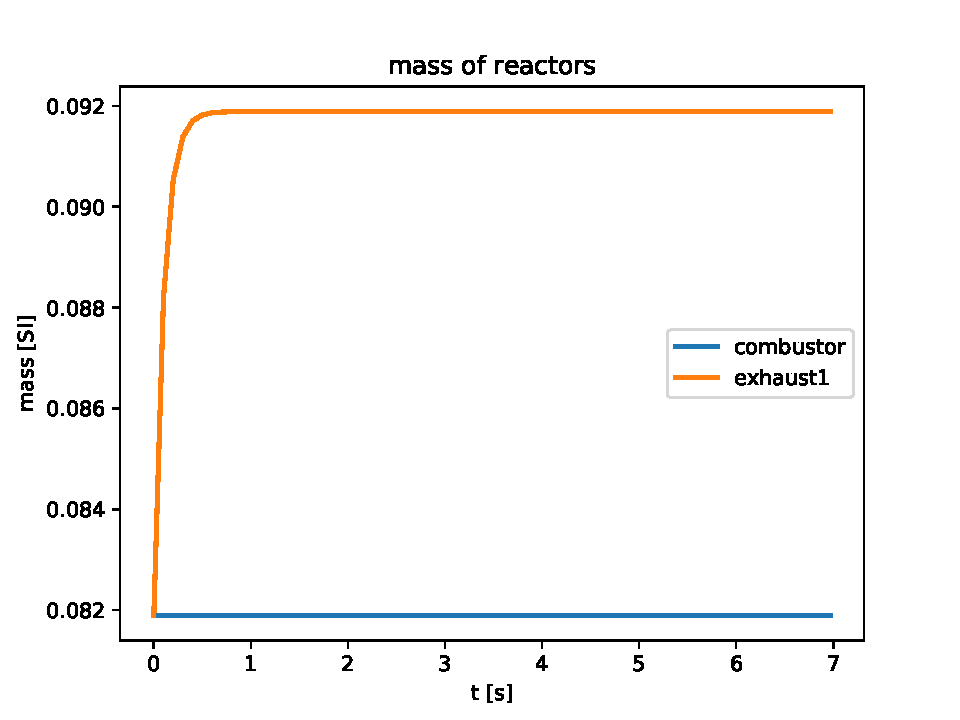
\includegraphics[scale=0.45]{examples/report/figures/mass.pdf}  
  \caption{Plot of mass produced by the \pyplume{}.}
  \label{fig:sub-first}
\end{subfigure}
\begin{subfigure}{.6\textwidth}
  \centering
  % include second image
  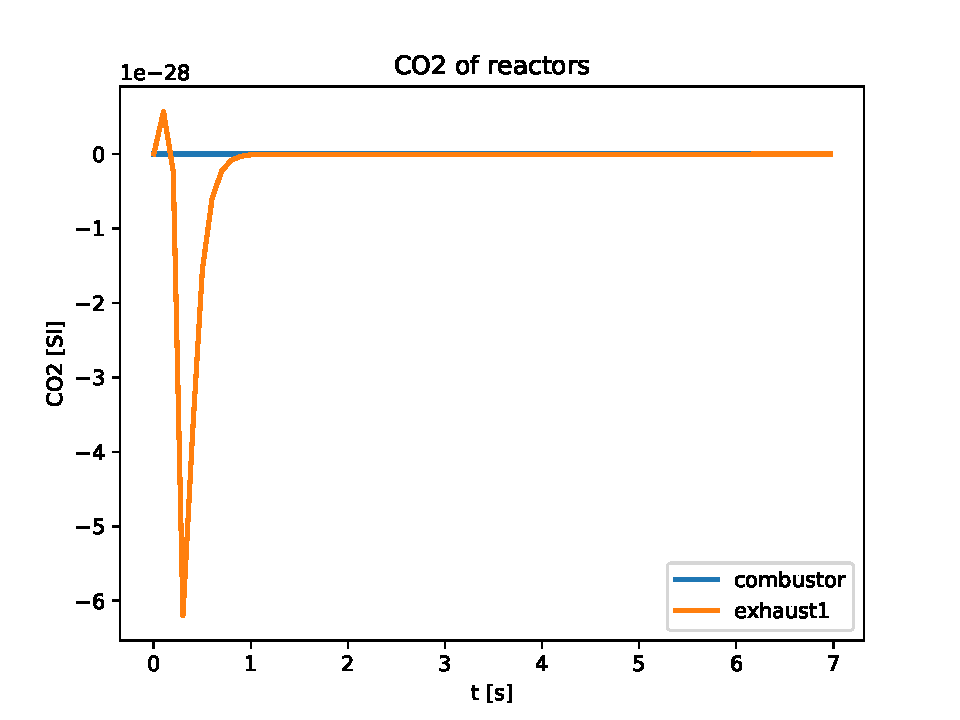
\includegraphics[scale=0.45]{examples/report/figures/CO2.pdf}  
  \caption{Plot of $CO_2$ produced by the \pyplume{}.}
  \label{fig:sub-second}
\end{subfigure}
\caption{Plots generated by \texttt{pyplume.figures}.}
\label{fig:plots}
\end{figure}

\subsection{\textbf{Script}}
These same results can be produced in a python script that looks something like this
\begin{codeblock}{Script interface to match the commandline example.}
\begin{lstlisting}[language=Python]
import pyplume
# Mechanism management
cti = 'test.cti'
pyplume.mech.mechFileAdd(cti) #Add mechanism file
# Model Use
pm = pyplume.model.PlumeModel.gridModel(mechs=[cti,'air.cti',cti])
pm.buildNetwork()
for t in np.arange(0.1,1.1,0.1):
    pm(t)
pm.steadyState()
#Plotting
fgk = pyplume.figures.figureGenerationKit("./simple.hdf5")
fgk.plotProperty(['CO2','mass'],save=True)
\end{lstlisting}
\label{code:script}
\end{codeblock}



\section{Conclusions \& Future Work}

In this paper, I have presented the basic functionality of \pyplume{} but it can be used for much more complicated scenarios. It consists of four currently implemented modules for modeling and graphing the results of exhaust reactor networks. These modules are \texttt{mech}, \texttt{model}, \texttt{figures}, \texttt{output}. With these modules and proper configuration of initial conditions, I should be able to run fairly complicated reactor network simulations with relative ease.

In the future, I hope to complete the package's fifth module which was intended to be statistical analysis of the results. I also hope to complete more extensive testing suites for the other modules and set up some kind of continuous integration. As it stands, the only real theory behind the code is that of Cantera's\cite{cantera}; I hope to include relevant exhaust modeling research in the form of class methods.

\bibliographystyle{plainurl}
\bibliography{references}

\end{document}
